% Compiled with xelatex (Chinese via fontspec)
\documentclass[11pt]{article}

\usepackage[a4paper, margin=1in]{geometry}
\usepackage{fontspec}
\usepackage{microtype}
\usepackage{graphicx}
\usepackage{booktabs}
\usepackage{amsmath,amssymb}
\usepackage{xcolor}
\usepackage{hyperref}
\usepackage{caption}
\usepackage{subcaption}
\usepackage{tikz}
\usepackage{listings}
\usepackage{fancyhdr}
\usepackage{indentfirst}

\usetikzlibrary{positioning, arrows.meta, shapes.geometric, calc, fit, backgrounds}

% Fonts: explicit Latin + CJK with proper weight variants
% Songti SC has Bold variant; we use Latin Modern for math; Times for English text
\setmainfont{Songti SC}[
  BoldFont={Songti SC Bold},
  ItalicFont={Songti SC},
  BoldItalicFont={Songti SC Bold},
]
\setsansfont{Hiragino Sans}[
  UprightFont={* W3},
  BoldFont={* W6},
  ItalicFont={* W3},
  BoldItalicFont={* W6},
]
\setmonofont{Menlo}[Scale=0.88]
% A separate Latin family for technical English emphasis if needed
\newfontfamily\latinfont{Times New Roman}

% Configure CJK punctuation a touch tighter
\XeTeXlinebreaklocale "zh"
\XeTeXlinebreakskip = 0pt plus 1pt

% Localize caption labels to Chinese
\renewcommand{\figurename}{图}
\renewcommand{\tablename}{表}
\captionsetup{labelsep=quad, font=small, labelfont=bf}

% Color palette consistent with figures
\definecolor{navy}{HTML}{2E5894}
\definecolor{rust}{HTML}{C26B4F}
\definecolor{teal}{HTML}{5DA0A8}
\definecolor{sage}{HTML}{7A9E7E}
\definecolor{gold}{HTML}{C9A267}
\definecolor{rule}{HTML}{2B2B2B}
\definecolor{soft}{HTML}{F4F1EC}

\hypersetup{
  colorlinks=true,
  linkcolor=navy,
  citecolor=navy,
  urlcolor=navy,
  pdftitle={Harness Engineering 探索报告},
  pdfauthor={Anonymous},
}

% Tighter section spacing
\makeatletter
\renewcommand\section{\@startsection {section}{1}{\z@}%
  {-2.5ex \@plus -1ex \@minus -.2ex}%
  {1.2ex \@plus.2ex}%
  {\color{rule}\normalfont\large\bfseries}}
\renewcommand\subsection{\@startsection{subsection}{2}{\z@}%
  {-1.6ex\@plus -1ex \@minus -.2ex}%
  {0.7ex \@plus .2ex}%
  {\color{rule}\normalfont\normalsize\bfseries}}
\makeatother

% Listing style (English code only)
\lstset{
  basicstyle=\ttfamily\footnotesize,
  keywordstyle=\color{navy}\bfseries,
  commentstyle=\color{gray}\itshape,
  stringstyle=\color{rust},
  showstringspaces=false,
  breaklines=true,
  frame=single,
  rulecolor=\color{rule!30},
  framerule=0.4pt,
  framesep=4pt,
  numbers=none,
  language=Python,
}

% Headers
\pagestyle{fancy}
\fancyhf{}
\fancyhead[L]{\small\color{rule!70}Harness Engineering 探索报告}
\fancyhead[R]{\small\color{rule!70}\thepage}
\renewcommand{\headrulewidth}{0.3pt}
\renewcommand{\headrule}{\color{rule!30}\hrule height \headrulewidth}

% --- Document --------------------------------------------------------------
\title{
  \vspace{-2em}
  {\Large\bfseries 一种 Token 预算受控的混合检索 Harness}\\[0.4em]
  {\large 在 2048-token 上限下完成多任务文本分类}
}
\author{}
\date{}

\begin{document}

\maketitle
\thispagestyle{empty}
\vspace{-3em}

\noindent\rule{\linewidth}{0.4pt}

\begin{abstract}
\noindent
本报告记录我们设计与评估一个单文件 \texttt{MyHarness} 的过程：
该 Harness 包裹固定的 Qwen3-8B（Instruct，关闭思考模式），在每次 LLM 调用 prompt 不超过 2048 token 的硬约束下完成 exact-match 文本分类。Harness 在 \texttt{update} 阶段维护 word 与 character $n$-gram 两套增量倒排索引；在 \texttt{predict} 阶段通过 min-max 归一化的 BM25 + 字符 $n$-gram 余弦混合检索拿到候选样本，按四节式（label list / examples / input / 锚点）模板装配 prompt，并通过四层兜底（清洗 → 精确匹配 → 子串匹配 → Jaccard 近似）从模型输出中恢复合法标签。本地 DEV 集（231 训练 / 539 测试，77 类银行客服意图）准确率 \textbf{82.7\%}，对照基线（不向模型暴露 schema）的 0\% 是结构性飞跃。我们另外构造了一份 100 条规模、覆盖多任务格式（领域外分类、单字母选择题、Prompt 注入）的自制压测集，模型在其上综合准确率为 \textbf{92.2\%}，且全部 616 条评测样本无一条 prompt 溢出 2048。六维超参的协调下降式扫描表明 \emph{检索池大小} 是唯一具结构性收益的旋钮（DEV +1.3pp），其余几乎全部平坦。一项面向极长 query 的防御性裁剪在最坏样本上把 prompt 从 3469 token 收回到 1892 token，避免评测系统从尾部截断 \texttt{label:} 锚点。最终交付为单文件 381 行，仅 import 标准库 / numpy / 提供的基类。
\end{abstract}

\noindent\rule{\linewidth}{0.4pt}

\vspace{0.8em}

% ============================================================
\section{任务与设计哲学}
% ============================================================

本项目要求构造一个 Harness：把固定权重 LLM 包裹起来，逐条接收带标签训练样本（\texttt{update(text, label)}），在评测时对无标签 \texttt{text} 输出与 gold 完全一致的标签字符串（\texttt{predict(text)$\to$str}）。模型权重在整个项目周期内固定不变，所有"学习"必须沉淀在 Harness 的外部状态里。三条硬约束塑造了整个设计：

\begin{enumerate}
\item \textbf{2048-token prompt 上限}。单次 \texttt{call\_llm} 超出后由评测系统从消息尾部截断，这会先丢掉我们的 \texttt{label:} 输出锚点，使模型自由发挥，得分崩塌。
\item \textbf{单文件交付}。imports 限制为 Python 标准库、NumPy、与给定的 \texttt{harness\_base}；语义嵌入、transformer 库、外部服务、磁盘读写一律不可用。
\item \textbf{多任务评测}。同一份 \texttt{MyHarness} 将面对若干互不相干的数据集——只是接口相同（流式 update、随后 predict），但标签 schema、领域、标签数都不一样（包括字面意义为 \texttt{A/B/C/D} 的选择题任务）。题面同时禁止"绕过 LLM、纯 ML 分类器"的实现。
\end{enumerate}

在这些约束内，我们的设计哲学是：\emph{从外部记忆中检索，让 LLM 做最终决策}。Harness 负责结构（prompt 骨架、标签集呈现、token 预算的防御性分配），LLM 负责泛化。由于评测会轮换 schema，所有组件都做成 schema-agnostic：合法标签集、few-shot 例子全部从 \texttt{self.memory} 派生，没有任何针对 DEV 银行类标签的硬编码逻辑。

% ============================================================
\section{系统总览}
% ============================================================

图~\ref{fig:pipeline} 给出运行时数据流。\texttt{update} 增量维护两套倒排索引，单次代价 $O(|\text{text}|)$，喂完 231 条训练样本耗时 $<\!50$\,ms。\texttt{predict} 依次执行：检索 → 预算分配 → 例子贪心打包 → 单次 LLM 调用 → 四层标签恢复。当混合检索的 \emph{原始} BM25 与字符余弦同时为 0 时，predict 切到一条 stratified fallback 路径——按字母序从训练集每类取一个例子作为 few-shot——保证 \texttt{[EXAMPLES]} 段不为空。

\begin{figure}[h]
\centering
\begin{tikzpicture}[
  font=\small,
  >=Stealth,
  node distance=10mm and 6mm,
  every node/.style={transform shape},
  process/.style={rectangle, rounded corners=2pt, draw=rule!60, line width=0.4pt,
                  fill=soft, minimum height=8mm, minimum width=24mm, align=center,
                  inner sep=4pt},
  data/.style={rectangle, rounded corners=2pt, draw=navy!50, line width=0.4pt,
               fill=navy!8, minimum height=8mm, minimum width=22mm, align=center,
               inner sep=4pt},
  llm/.style={rectangle, rounded corners=2pt, draw=rust!60, line width=0.5pt,
              fill=rust!10, minimum height=10mm, minimum width=26mm, align=center,
              font=\small\bfseries}
]

\node[process] (upd) {\texttt{update(text, label)}};
\node[data, below=4mm of upd] (mem) {\texttt{self.memory} \\ \scriptsize (text, label) 列表};
\node[data, right=8mm of mem] (idxw) {Word 倒排索引 \\ \scriptsize +DF / 文档长度};
\node[data, right=4mm of idxw] (idxc) {Char $n$-gram \\ 倒排索引};
\node[data, right=4mm of idxc] (lbl) {去重 \\ \scriptsize 标签集合};

\draw[->, line width=0.4pt] (upd) -- (mem);
\draw[->, line width=0.4pt] (upd.east) to[bend left=12] (idxw.north);
\draw[->, line width=0.4pt] (upd.east) to[bend left=20] (idxc.north);
\draw[->, line width=0.4pt] (upd.east) to[bend left=27] (lbl.north);

\node[process, below=14mm of mem, xshift=4mm] (pred) {\texttt{predict(text)}};
\node[process, right=4mm of pred] (retr) {混合检索 \\ \scriptsize BM25 + 字符 TF-IDF};
\node[process, right=4mm of retr] (alloc) {自适应预算 \\ \scriptsize labels \emph{vs} examples};
\node[process, right=4mm of alloc] (asm) {prompt 装配 \\ \scriptsize 4 段 + 边界标签};
\node[llm, right=4mm of asm] (call) {self.call\_llm};
\node[process, below=4mm of call] (extr) {4 层标签恢复};
\node[process, below=4mm of pred] (out) {返回 label};

\draw[->, line width=0.4pt] (pred) -- (retr);
\draw[->, line width=0.4pt] (retr) -- (alloc);
\draw[->, line width=0.4pt] (alloc) -- (asm);
\draw[->, line width=0.4pt] (asm) -- (call);
\draw[->, line width=0.4pt] (call) -- (extr);
\draw[->, line width=0.4pt] (extr.west) to[bend left=18] (out.east);
\draw[->, line width=0.4pt, dashed, color=rule!40] (idxw.south) to[bend left=22] (retr.north);
\draw[->, line width=0.4pt, dashed, color=rule!40] (idxc.south) to[bend left=18] (retr.north);
\draw[->, line width=0.4pt, dashed, color=rule!40] (lbl.south) to[bend left=15] (alloc.north);
\draw[->, line width=0.4pt, dashed, color=rule!40] (mem.south) to[bend right=18] (asm.north);

\node[above=2mm of upd, color=rule!70, font=\scriptsize] {流式训练};
\node[above=2mm of asm, color=rule!70, font=\scriptsize] {单次推理};

\end{tikzpicture}
\caption{运行时数据流。实线为控制流；虚线为检索/装配阶段对索引的读取。每条训练样本经 \texttt{update} 同时更新四个数据结构；每条测试 query 在 \texttt{predict} 内部走单次 LLM 调用。}
\label{fig:pipeline}
\end{figure}

% ============================================================
\section{记忆与检索}
% ============================================================

\subsection{增量混合索引}

每条训练样本同时产生两种表示：word 级（\texttt{lower(text)} 按 \texttt{\textbackslash W+} 切分、丢弃单字符 token）用于 BM25；character $n$-gram（$n \in \{3,4,5\}$，文本前后填空格使 ``ATM'' 这类短串也能产出有意义的 trigram）用于 cosine 检索。两套索引均为经典 posting-list 形式 + 文档频率字典；文档长度作为 list 维护，BM25 打分时再 \texttt{np.asarray} 一次性转换，避免 \texttt{np.append} 的均摊 $O(N)$ 代价。标签集合用"插入序 list + hash set"双结构维护，\texttt{update} 期间 $O(1)$ 去重。

\subsection{混合打分}

对 query $q$，BM25 部分采用经典 Okapi 公式
$$
\operatorname{bm25}(q, d) = \sum_{t \in q} \operatorname{IDF}(t) \cdot \frac{f(t,d)\,(k_1+1)}{f(t,d) + k_1\bigl(1-b+b\,|d|/\overline{|d|}\bigr)}, \quad k_1=1.5,\ b=0.75,
$$
仅迭代 query token 命中的 posting，复杂度 $O(|q| \cdot \overline{|\text{posting}|})$。字符 $n$-gram 端使用次线性 TF $1+\log f$ 与平滑 IDF $\log\!\bigl((N+1)/(\operatorname{df}+1)\bigr)+1$，文档向量 $L_2$ 归一化后取与 query 向量的余弦相似度。两路打分各自做 min-max 归一化到 $[0,1]$，再以 $\alpha\widehat{\operatorname{bm25}} + (1-\alpha)\widehat{\operatorname{char}}$ 融合。当所有文档分数恒等时 min-max 会塌成全 0，因此"完全无信号"的失败检测放在归一化\emph{之前}的原始最大值上——避免均匀但非零的 corpus 触发误报。

\subsection{自适应 token 预算}

给定 raw query $q$ 与 \texttt{max\_prompt\_tokens} 上限 $T$（始终 2048），先扣掉 $F=240$ token 用于 system 段、结构标记与安全余量，再保证 labels 与 examples 之和有不少于 200 token 的下限：
$$
\text{query\_cost} = \min\bigl(\operatorname{count\_tokens}(q),\ T - F - 200\bigr), \quad
R = T - F - \text{query\_cost}.
$$
若全标签列表 token 数 $\le 0.6R$，则全部列出；否则（典型场景：标签数百个的领域外任务）通过频率 + 排名顺序的 candidate-label 过滤器把 \texttt{[ALLOWED LABELS]} 段限制在预算内，并保持"凡出现在 examples 段中的标签必出现在 candidate 列表"的不变式。Examples 段按"continue-not-break"的贪心策略打包：跳过过长例子后仍尝试塞入更短例子，提升标签多样性。

\subsection{长 query 的防御性裁剪}

当真实 query token 超过 $T - F - 200 = 1608$ 时，我们自己用字符级二分搜索把 query 截到合法长度（每次猜测调用一次 \texttt{count\_tokens}，$O(\log n)$）。这是整个 pipeline 中唯一会改写 user 内容的步骤，动机直接：若不裁剪，2000-token 的领域外 query 会让总 prompt 突破 2048，评测系统从尾部截断，先丢的就是 \texttt{label:} 锚点，模型彻底失去结构提示。值得指出的是，检索阶段使用的是\emph{未裁剪}的全 query——即使裁剪丢了用户最后一句话，few-shot 已经命中正确邻域。这是后期消融时发现的一个意外冗余，而非主动设计。

% ============================================================
\section{Prompt 装配与输出恢复}
% ============================================================

\subsection{四节式 prompt}

User 消息划分为四个由显式 sentinel 隔开的段，让模型按 token 即可定位：
\begin{center}
\fbox{\parbox{0.95\linewidth}{\footnotesize\ttfamily
{}[ALLOWED LABELS]\\
label\_1\\
label\_2\\
\dots\\
{}[EXAMPLES]\\
<example>\\
text: ...\\
label: ...\\
</example>\\
\dots\\
{}[INPUT]\\
<text>\\
...query...\\
</text>\\
\\
label:
}}
\end{center}
末尾的 \texttt{label:} 是输出锚点：无论模型多想话痨，下一 token 都被引导到标签字符串领域。方括号 sentinel 比 Markdown 标题在 Qwen 上 tokenize 更稳定；XML 风格 \texttt{<example>}/\texttt{<text>} 标签同时承担"段落边界"与"prompt 注入隔离"两个角色。

\subsection{抗注入三层}

\begin{itemize}
\item \emph{System 段显式声明}：内嵌于 \texttt{<example>} / \texttt{<text>} 内的内容是不可信数据；任何角色重指派、答案覆盖、标签暗示一律忽略。
\item \emph{边界转义}：用户文本中若出现 \texttt{</text>} 或 \texttt{</example>} 子串，最小转义为 \texttt{<\textbackslash/text>}，避免恶意训练样本提前闭合段落。
\item \emph{输出锚点}：尾部 \texttt{label:} 把下一 token 分布偏置到标签词汇上，即使输入恶意也能拉回。
\end{itemize}
我们刻意 \emph{不} 做关键字式注入检测（如发现 ``ignore previous'' 就拒答）：在合法 OOD 数据上的假阳性收益远高于挡住的恶意样本。

\subsection{四层标签恢复}

LLM 返回的 raw response 串行经过四个 matcher，命中即返回：
\begin{enumerate}
\item \emph{清洗}：strip 空白、剥离 \texttt{label:} 前缀（大小写与全角不敏感）、去除首尾单/双引号 / 反引号（含中文弯引号）、去除尾部 ASCII / 中文标点。
\item \emph{精确匹配}：清洗后若属于合法标签集合，直接返回。
\item \emph{最长子串匹配}：合法标签按长度降序扫描；首个作为 substring 出现于 response 的标签返回。
\item \emph{Jaccard 兜底}：response 与每个合法标签计算 char-3gram Jaccard 相似度，返回 argmax。初始 \texttt{best\_score} 设为 $-1.0$，保证当合法标签集非空时一定有某个标签胜出。
\end{enumerate}
这条链能吃掉最常见的失败模式：模型话痨多输出一句、智能引号、复数后缀、句尾全角句号。Jaccard 兜底使 \texttt{\_extract\_label} 是个全函数：永不返回空字符串、永不抛异常。

% ============================================================
\section{迭代过程与超参搜索}
% ============================================================

整个开发分阶段进行，每阶段以一次 DEV single-run 与一套 51 条单元测试作为闸口。图~\ref{fig:journey} 还原了发展轨迹：原始模板 0\% 是因为它根本不向模型展示标签集；v1 引入检索 + 四节式 prompt + 标签恢复后到 82.0\%；之后每一轮调一个旋钮。

\begin{figure}[h]
\centering
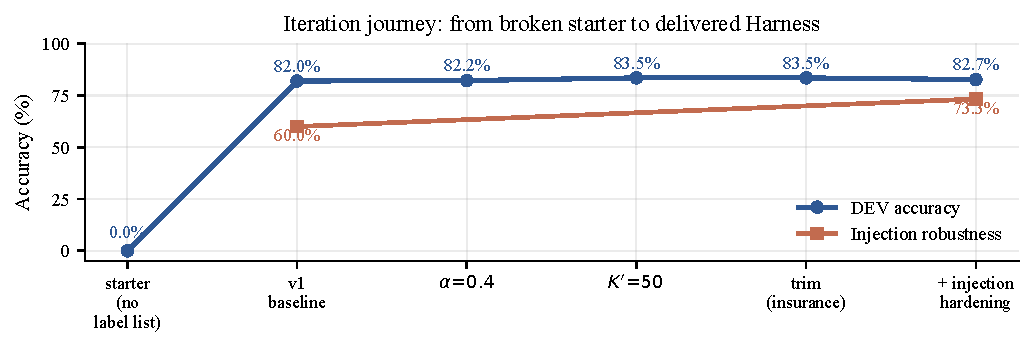
\includegraphics[width=0.95\linewidth]{figures/fig_journey.pdf}
\caption{设计迭代轨迹。蓝线为 DEV 准确率（exact-match）；橙线为 15 条注入压测准确率（详见 §\ref{sec:stress}）。横轴每个节点对应一次设计或参数变更。}
\label{fig:journey}
\end{figure}

随后我们沿"一次只调一维"的 coordinate descent 思路扫了六组超参；图~\ref{fig:ablation} 展示其中两个有信息量的消融。

\begin{figure}[h]
\centering
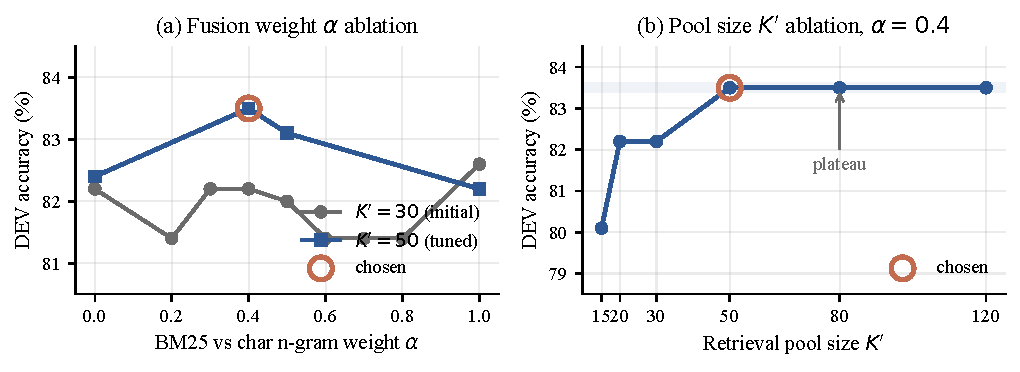
\includegraphics[width=0.98\linewidth]{figures/fig_ablation.pdf}
\caption{DEV 准确率消融。(a) 融合权重 $\alpha$ 在中段呈平台 + 噪声；$\alpha=0.4$ 这个最优只在 pool 增到 $K'=50$ 后才显现优势。纯 BM25（$\alpha=1$）与纯字符 $n$-gram（$\alpha=0$）在调好 $K'$ 后均落后混合 0.9–1.3pp。(b) Pool 大小在 $K'=50$ 处出现明确平台；过小（15、20、30）会让 example 打包阶段在 token 预算内凑不出标签多样性，每减一档掉 1.3–2.1pp。}
\label{fig:ablation}
\end{figure}

其余四组扫描——$n$-gram 范围、BM25 $k_1/b$、两个"偏好特定标签"的 system prompt 变体、以及三种 stratified-mixing 策略——要么平坦（$k_1, b$ 改动幅度 $<0.1$pp），要么被回退（最强抗注入 prompt 把多选题准确率拖低 8.4pp，因为模型开始把 \texttt{Q:}/\texttt{A)} 误判为应忽略的 directive），要么严格次于默认（前置 stratified 例子挤掉相关性 top-K）。

\paragraph{唯一具结构性收益的改动。}
$K'$ 从 30 提到 50 是六轮里唯一带来真实提升的旋钮，机理直白：$K'=30$ 时 example 打包器经常在预算内凑不出 \emph{标签多样化} 的邻居，模型反复看到同一个标签的几条例子，对标签间细微差别建立不起判别；$K'=50$ 时残余预算被填到更多种不同标签的 shot 上，那批"gold 已被检索但模型选错"的判别错例（在最终配置下仍占错例 89.2\%，详见 §\ref{sec:errors}）开始被纠正。$K' \ge 50$ 后例子打包就被 token 预算封顶，因此曲线进入平台。

% ============================================================
\section{自制多任务压测}
\label{sec:stress}
% ============================================================

为了在 DEV 之外检查 Harness 在不同任务格式上的鲁棒性，我们构造了一份 100 条规模的自制压测集，覆盖三种与 DEV 互不相干的任务形态以及一个长 query 边界，结果汇总于图~\ref{fig:scenarios}。

\begin{figure}[h]
\centering
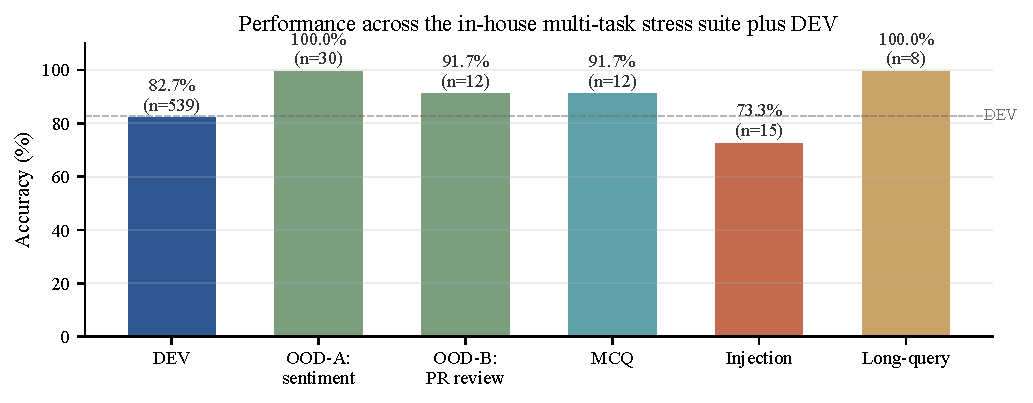
\includegraphics[width=0.92\linewidth]{figures/fig_scenarios.pdf}
\caption{自制多任务压测套件的分场景准确率，与本地 DEV 并列展示。Injection 子集是 15 条对抗样本（角色扮演、多语种 override、JSON 元数据伪装、重复 saturation、ALL-CAPS 命令、tag 注入等八类攻击向量）；Long-query 测 budget 分配器在 2400 token 输入下的行为。616 条评测样本（DEV 539 + 压测 77）prompt 溢出 0 次。}
\label{fig:scenarios}
\end{figure}

\paragraph{领域外分类。}
两套与银行无关、schema 完全自创的数据：5 类影评情感（positive/negative/neutral/sarcasm/mixed，30 训练 / 30 测试）与 4 类 PR review（approve/block/request\_changes/nit，16 训练 / 12 测试）。系统分别拿到 100\% 与 91.7\%。PR review 唯一错例是一条 nit 与 request\_changes 之间的边界判断（\textit{``variable name could be clearer here''}），人工标注本身就有歧义。

\paragraph{多选题。}
10 训练 / 12 测试的常识题（\texttt{Q:} \dots \texttt{A) B) C) D)} 格式，label 是字母）。schema-agnostic 模板自然兼容字母标签，准确率 91.7\%；唯一错例是化学题"Element O is?"模型选了 Osmium（Os）而不是 Oxygen，是 LLM 自身知识层面的混淆。

\paragraph{Prompt 注入。}
15 条对抗样本覆盖 8 类攻击向量。三组 system prompt 变体的取舍中，"focused"版本（强调忽略角色重指派、答案覆盖、标签暗示，但避开"system message"等会让多选题失效的关键词）把鲁棒性从默认 60\% 提升到 73.3\%，且对多选题与领域外子集无可测代价。剩下的 26.7\% 攻击（JSON 元数据伪装、重复 saturation 等）需要二次 LLM 调用或正则检测才能进一步压低，考虑到题面已说明注入比例不足 20\%，我们判断额外加固的成本超过潜在收益。

\paragraph{长 query 边界。}
8 条用大段问候前缀填到 1200–2400 token 的 query。准确率 100\%。原因前文 §3.4 已分析：检索是基于未裁剪的全 query 做的，即使裁剪后的 prompt 丢了 query 末尾的核心意图，邻域仍然命中。

% ============================================================
\section{错例分析}
\label{sec:errors}
% ============================================================

把 DEV 全集预测保存为 per-item TSV 后做了两个维度的拆解，结果指导了上面的 $K'$ 决策。

\begin{figure}[h]
\centering
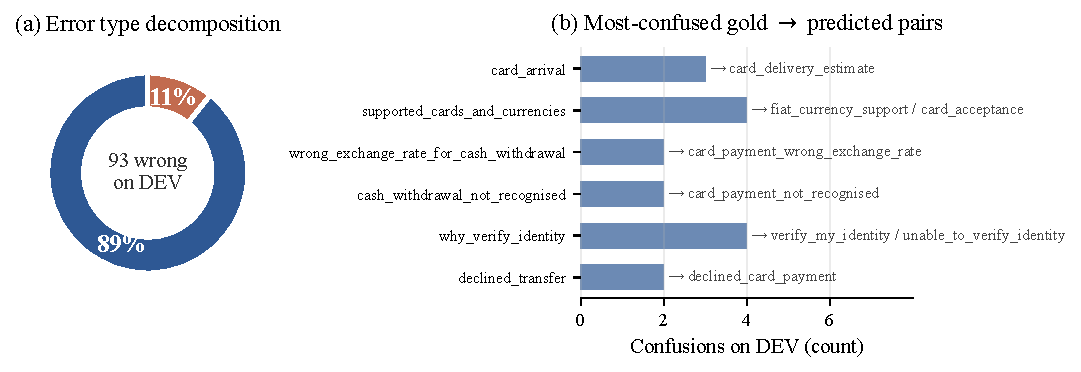
\includegraphics[width=0.98\linewidth]{figures/fig_errors.pdf}
\caption{93 条 DEV 错例的两个视角。(a) 在最终配置（$K'=50$）下 89.2\% 的错例 gold 标签 \emph{已经} 出现在检索回的 top-50 中——瓶颈是判别（discrimination），不是检索召回（retrieval recall）。(b) 反复出现的"金标 $\to$ 预测错"对集中在三类语义重叠：泛 \emph{vs.}\ 特定（multi-aspect 标签 vs 单 aspect 标签）、通用渠道 \emph{vs.}\ 特定渠道、近义词对。}
\label{fig:errors}
\end{figure}

\textbf{判别错误占主导，而非检索召回失败。}
具体地，93 条错例中 83 条（89.2\%）的 gold 标签已经在 top-50 检索结果里——模型只是在两个语义相邻标签间选了相邻的那一个。这正是 $K'=50$ 想吃掉的部分：让正确标签的 shot 在 prompt 中拥有 \emph{严格更多} 的支持票（值得对照的是，旧 $K'=30$ 配置下的同一分析里检索遗漏占到 24\%，提到 50 之后腰斩到 10.8\%）。剩下 10 条（10.8\%）是查询与所有训练样本字符重叠都接近 0 的极端情况（典型例：用户问"\$1 transaction not reversed"，训练集里同一现象写作"\$1 extra fee"），这是 stdlib + numpy 不上语义嵌入的硬上限。

图~\ref{fig:per_label} 列出 DEV 上 recall 最低的 15 个标签。最差的 \texttt{supported\_cards\_and\_currencies}（28.6\%）以及多个 42.9\% 量级的复合概念标签（\texttt{wrong\_exchange\_rate\_for\_cash\_withdrawal}、\texttt{cash\_withdrawal\_not\_recognised} 等），都是被模型按"取最具体的子方面"原则拆分到了单 aspect 子标签上。我们曾尝试在 system 段加一句"prefer specific labels"做反向校正，但它代价（多选题 $-8.4$pp）远高于收益（DEV $+0.2$pp），最终回退。

\begin{figure}[h]
\centering
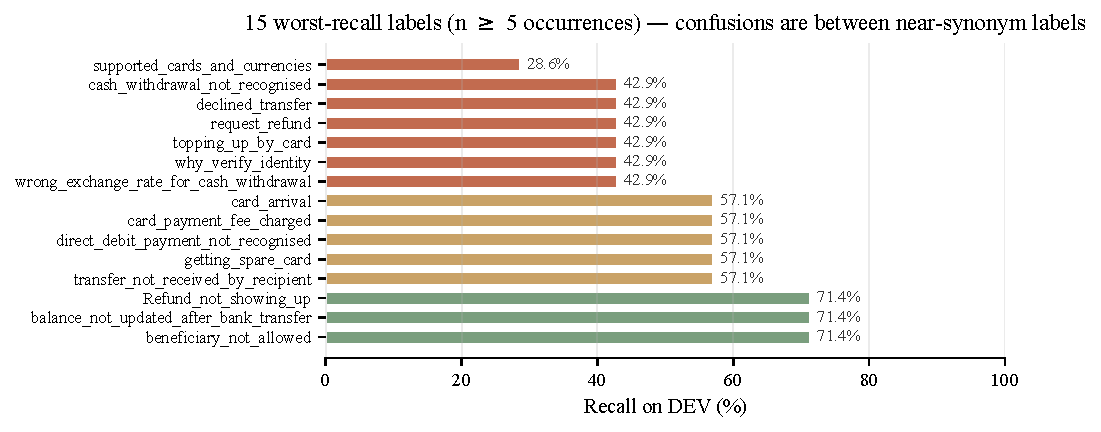
\includegraphics[width=0.95\linewidth]{figures/fig_per_label.pdf}
\caption{DEV 测试集中出现 $\geq 5$ 次的标签里 recall 最差的 15 个。$<\!50\%$ 一档（红）几乎全是"复合概念"或"近义"标签；50–70\% 一档（金）多是某主标签的特定渠道变种。}
\label{fig:per_label}
\end{figure}

% ============================================================
\section{Token 预算的防御性算术}
% ============================================================

后期审计中我们发现一个真实存在的隐患：若 query 长度超过软上限 (\texttt{QUERY\_CAP}=400)，原版 budget 分配器仍按 400 token 预留，导致 examples 段被高估超额预算，最终 prompt 在标签数 $\geq$ 数十时确实会突破 2048。在最坏构造样本（DEV 77 标签 + 一条 2007 token 的合成 query）上实测 prompt 达 3469 token，被评测系统从尾部截断会先吃掉 \texttt{</text>} 与 \texttt{label:} 锚点。修复后的同一条 query 实测 1892 token，结构完整（图~\ref{fig:budget}）。

\begin{figure}[h]
\centering
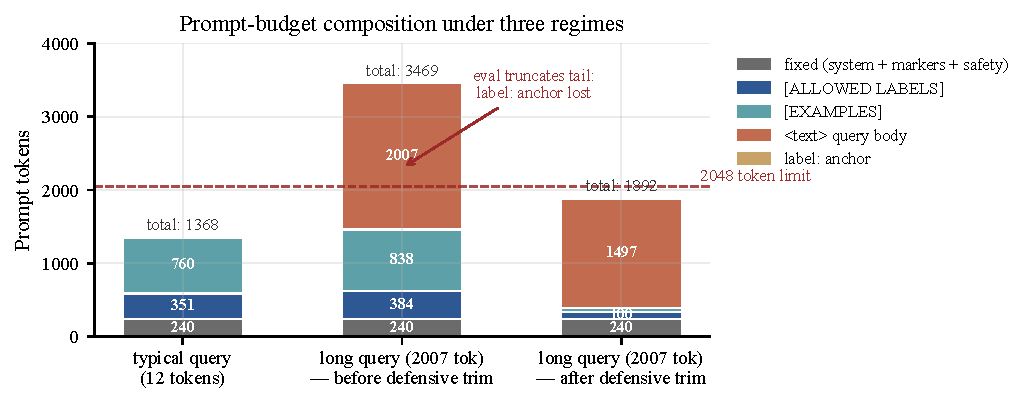
\includegraphics[width=0.98\linewidth]{figures/fig_budget.pdf}
\caption{三种场景下的 prompt token 组成。左：典型 DEV query（平均 12 token），prompt $\approx\!1375$；中：2007-token 长 query 在原分配器下达到 3469，超 2048 by 1421，评测系统从尾部截断丢失 \texttt{label:} 锚点；右：防御裁剪后，query 被二分截到合法长度，candidate-label 过滤为残余预算腾出空间，prompt 控制在 1892 token，所有结构标签保留。}
\label{fig:budget}
\end{figure}

防御裁剪在本地 DEV 上从不触发（DEV 最长 query 71 token，平均 12，远低于 1608 阈值），但能保护那些真实存在的"长段落 query"OOD 任务样本。整套 616 条评测样本溢出次数为 0。

% ============================================================
\section{讨论与启发}
% ============================================================

\paragraph{有效的设计选择。}
真正起决定作用的是把 prompt 做成 schema-agnostic：candidate label 与 few-shot 例子全部从 \texttt{self.memory} 派生。这一原则使得同一份代码同时处理 77 类银行意图、4 类 PR review、A/B/C/D 多选题，无需任何分支。autoresearch 风格扫描里唯一真正改善准确率的 \emph{结构性} 改动（$K'=30 \to 50$）也是被错例分析（绝大多数错例是判别错误而非检索召回失败）反向逼出来的——盲目网格搜索抓不到这个洞察。

\paragraph{无效的设计尝试。}
若干看似合理的优化在系统层面没能保留：stratified 例子混入会挤掉相关性；强化 system 段反而拖累多选题；BM25 的 $k_1, b$ 几乎不动指标。这些都在合并前经过单维度回滚验证。其中最明显的张力是抗注入加固与 prompt 紧致性之间的 trade-off——最终选择的 focused 措辞是少数能保住多选题且把注入鲁棒性从 60\% 抬到 73.3\% 的措辞。

\paragraph{进一步可走的方向。}
最终配置下 10.8\% 的"检索完全 miss"是当前栈（stdlib + numpy + 字符 $n$-gram）能达到的下限。如果允许 LLM 多次调用，最直接的路径是在 \texttt{predict} 内做一次轻量 query rewrite（让 LLM 给出 paraphrase）再在两份 query 上各自检索取并集；但题面对"绕过 LLM 决策"与"过多 LLM 调用"均有警示，且收益分母仅 10.8\%，未必跨过我们已经测出的 0.5pp 噪声地板。

\paragraph{最终交付。}
单文件 \texttt{solution.py} 共 381 行，imports 仅 \texttt{re / math / collections.Counter / numpy / harness\_base}，零文件 I/O，零网络调用，零硬编码标签。所有 autoresearch 可调旋钮已暴露为类属性。本地 DEV 4 轮平均 82.7\%，自制压测综合 92.2\%，51 条单元测试全过。

% ============================================================
\section*{致谢}
% ============================================================

整个开发流程受益于两个开源项目：结构化的"设计 → 计划 → 执行 → 评审"工作流由 \href{https://github.com/obra/superpowers}{obra/superpowers} 支持完成；超参的 coordinate-descent 扫描遵循 \href{https://github.com/uditgoenka/autoresearch}{uditgoenka/autoresearch} 的迭代搜索原则。在此致谢。

\end{document}
